\section{Einleitung}
\label{sec-1}

\subsubsection*{Parameterabhängige Probleme}
\label{Parameterabhängige Probleme}

\begin{bsp}[Parameterabhängige PDE]
	Sie $\Omega \subseteq \R^d$ polygonales Gebiet. Zu Parametervektor $\mu \in \mathcal{P} \subset \R^p$ aus einer Menge $\mathcal{P}$ von "`erlaubten"' Parametern ist eine Funktion (z.\,B. "`Temperatur"') $u(\mu): \Omega \rightarrow \R$, s.\,d.:
	\begin{align*}
		\nabla \cdot (\kappa(\mu) \nabla u) &= q(\mu) & \text{in } \Omega \\
		u(\mu) &= 0 & \text{auf } \delta\Omega
	\end{align*}
	mit $\kappa(\mu) : \Omega \rightarrow \R$ (z.\,B. "`Wärmeleitungskoeffizient"') \\
	und $q(\mu) : \Omega \rightarrow \R$ (z.\,B. "`Wärmequelle/-senke"') \\
	
	z.\,B. $q(x;\mu) := \begin{cases}
			1 & \text{für } x \in \Omega_q \\
			0 & \text{sonst}
		\end{cases}$
\\

Weiter kann Ausgabe erwünscht, z.\,B. mittlere Temperatur
	\[
		s(\mu) = \frac{1}{|\Omega_s|} \int u(x; \mu) \,dx
	\]
	
\begin{figure}[H]
  \centering\small
    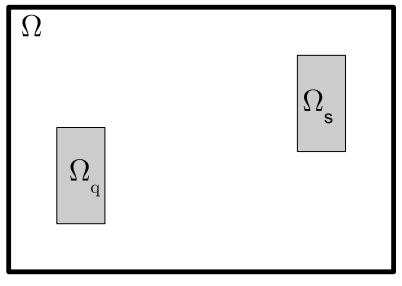
\includegraphics[width = 0.5 \textwidth]{Bilder/MittlereTemp.png}
  \caption{Beispiel Wärmeleitung mit Quelle $\Omega_q$ und Messbereich $\Omega_s$}{(aus B. Haasdonk, Reduzierte-Basis-Methoden, Skript zur Vorlesung SS 2011, Universität Stuttgart, IANS-Report 4/11, 2011.)}
  \label{fig:MittlereTemp}
\end{figure}
\end{bsp}

\begin{bsp}[Parametrisches stationäres System]
Zu Parameter $\mu \in \mathcal{P} \subseteq \R^p$ ist Zustandsvektor $u(\mu) \in \R^n$ und Ausgabe $s(\mu) \in \R^k$ gesucht, s.\,d.:
\begin{align*}
	0 &= A(\mu) \cdot u(\mu) + B(\mu) w(\mu) \\
	s(\mu) &= l(\mu) \cdot u(\mu)
\end{align*} 
mit parameterabhängigen Matrizen $A(\mu) \in \R^{n\times n}, B(\mu) \in \R^{n\times m}, C(\mu) \in \R^{k \times n}$ mit Eingabevektor $w \in \R^m$.
\end{bsp}

\subsubsection*{Schwache Formulierung in Hilberträumen}
\label{Schwache Formulierung in Hilberträumen}

Sie $X$ reeller Hilbertraum (reel, seperabel). Zu $\mu \in \mathcal{P}$ ist gesucht ein $u(\mu) \in X$ und $s(\mu) \in \R$
\begin{align*}
	a(u(\mu),v; \mu) &= f(v; \mu) \\
	s(\mu) &= l(u(\mu); \mu) & \forall v \in X
\end{align*}
Mit Bilinearform $a(\pdot,\pdot; \mu)$ und Linearform $f(\pdot; \mu)$, $l(\pdot; \mu)$. Beide Beispiele lassen sich so formulieren.

z.\,B. 1.1: 
\begin{align*}
	X=H_0^1(\Omega):=\{f\in L^2(\Omega) | \pd{x_i}& f \in L^2(\Omega), f_{|\delta\Omega} = 0\} \\
	\underbrace{\int_{\Omega} \kappa (x; \mu) \nabla u(x; \mu) \cdot \nabla v(x) dx}_{a(u(\mu),v; \mu)} &= \underbrace{\int_{\Omega} q(x; \mu) \cdot v(x) dx}_{f(v; \mu)} &\forall v \in X \\
	s(\mu) = \frac{1}{|\Omega_s|} \int_{\Omega_s} u(x; \mu) &=: l(u(\mu); \mu)
\end{align*}

Zu Bsp. 1.2 ($k=1$, "`single output"') \qquad $X = \R^n$
\begin{align*}
	\underbrace{v^TA(\mu)u(\mu)}_{a(u(\mu),v; \mu)} &= \underbrace{-v^TBw}_{f(v; \mu)} \\
	s(\mu) &:= \underbrace{C(\mu)u(\mu)}_{l(u(\mu); \mu)}
\end{align*}

In der Vorlesung werden weitere Verallgemeinerungen zu $a:X_1 \times X_2 \rightarrow \R$ mit $X_1 \neq X_2$, nichtlinear und instationäre Probleme behandelt.

\subsection{Modellreduktion}
\label{Modellreduktion}

\subsubsection*{Grundidee/Motivation}
\label{Grundidee/Motivation}

\begin{itemize}
	\item $\mathcal{M}:= \{u(\mu) | \mu \in \mathcal{P}\} \subset X$ für $\mathcal{P} \subseteq \R^p$ ist die durch $\mu$ parametrisierte Lösungsmannigfaltigkeit.
	\item $X$ ist im allgemeinen $\infty$-dimensional Sobolev-Raum) oder endlich- aber  sehr hochdimensional (FEM, FV, FD-Raum). $\mathcal{M}$ ist aber höchstens $p$-dimensional. \\
	$\Rightarrow$ Motivation für Suche nach einem niedrigdimensionalen Teilraum $X_n \subseteq X$ zur Approximation von $\mathcal{M}$ und einer Approximation $u_N(\mu) \approx u(\mu), u_N(\mu) \in X_N$
	\item Insbesondere bei Reduzierten-Basis-Methoden (RB-Methoden): \\
	$X_N$ durch Beispiellösungen erzeugt, sog. "`Snapshots"' \\
	$X_N \subseteq \op{span}\{u(\mu_1),...,u(\mu_n)\}$ für geeignete Parameterwerte $\mu_i \in \mathcal{P}$. \\
	Ziel ist außerdem Fehlerkontrolle durch Schranken $\Delta_N(\mu)$: \\
	\[
	||u(\mu) - u_N(\mu)|| \le \Delta_N(\mu)
	\]
\end{itemize}

\subsubsection*{Illustration}

\begin{figure}[H]
  \centering\small
    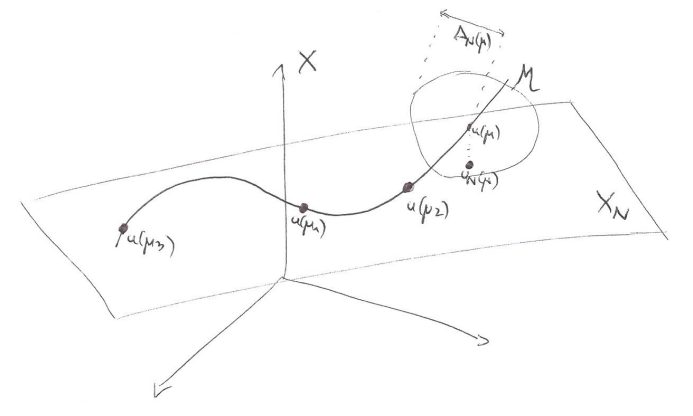
\includegraphics[width = 0.7 \textwidth]{Bilder/IllustrationM.png}
  \caption{Parametrisierte niedrigdimensionale Lösungsmenge}{(aus dem Online-Skript von Prof. Dr. Haasdonk zu Reduzierte Basen 2015)}
  \label{fig:IllustrationM}
\end{figure}

\begin{bsp}
	Gesucht ist $u(\mu) \in C^2([0,1])$ mit 
	\begin{align*}
		(1 + \mu) u'' &= 1 & \text{auf} (0,1) \\
		u(0) &= u(1) = 1
	\end{align*}
	Für $\mu \in [0,1] =: \mathcal{P} \subseteq \R$. Spezielle Lösungen ("`Snapshots"')
	\begin{align*}
		\mu &= 0 \Rightarrow u_0(x) = u(x; \mu = 0) = \frac{1}{2} x² - \frac{1}{2} x + 1 \\
		\mu &= 1 \Rightarrow u_1(x) = u(x; \mu = 1) = \frac{1}{4} x² - \frac{1}{4} x + 1 \\
	\end{align*}
	RB-Raum: $X_N := \op{span}(u_0,u_1)$
	Reduzierte Lösung gegeben durch
	\begin{align*}
		u_N(\mu) &:= \alpha_0(\mu)u_0 + \alpha_1(\mu)u_1 \\
		\alpha_0 (\mu) &= \frac{2}{\mu + 1} - 1 ; \qquad \alpha_1(\mu) = 2 - \frac{2}{\mu + 1}
	\end{align*}
	Diese erfüllt 
	\[
	 ||u_N(\mu) - u(\mu)||_{\infty} = \sup\limits_{\mu} ||u(\mu) - u_N(\mu)|| = 0
	\]
	ist somit exakt. $\mathcal{M}$ ist enthalten in 2-dimensionalem Unterraum $X_N$: Genauer $\alpha_0 + \alpha_1 = 1,\, 0 \le \alpha_0,\, \alpha_1 \le 1$, also ist $\mathcal{M}$ Menge der Konvexkombinationen von $u_0$, $u_1$.
\end{bsp}

\subsubsection*{Begriffe}
\label{Begriffe}

\begin{itemize}
	\item Eine PDE ist ein \emph{analytisches} Modell, welches die \emph{exakte Lösung} $u(\mu) \in X$ in einem typischerweise $\infty$-dimensionalen Funktionenraum $X$ charakterisiert.
	\item Ein \emph{detailliertes Modell} (auch \emph{hochdimensionales Modell}) ist ein Berechnungsverfahren oder charakterisiert eine Approximation $u(\mu) \in X$ in hochdimensionalen Raum mit sehr allgemeinen Approximationseigenschaften. (z.\,B. FEM/FV/FD, dim $X = 10^3 - 10^8$).
	In dieser Vorlesung kann $u(\mu)$ sowohl eine analytische als auch eine detaillierte Lösung darstellen.
	\item Ein \emph{reduziertes} Modell ist ein Berechnungsverfahren bzw. eine Charakterisierung einer reduzierten Lösung $u_N(\,u)$ in einem sehr problemangepassten Raum $X_N$ (dim $X_N = 1 - 10^3$).
	\item \emph{Modellreduktion} beschäftigt sich mit Methoden der Erzeugung reduzierter Modelle und Untersuchung ihrer Eigenschaften
	\item Modellreduktion ist ein modernes Gebiet der angewandten Mathematik und Ingenieurwissenschaften (Schwerpunkt in SimTech PN3, MOR-Seminar)
\end{itemize}

\subsubsection*{Anwendungen für parametrische reduzierte Modelle}
\label{Anwendungen für parameterische reduzierte Modelle}

"`Kleinere"' Modelle stellen geringere Anforderungen an Rechenzeit und Speicher, daher Einsatz in:

\begin{itemize}
	\item "`multi-query"'-Kontext, d.\,h. Vielfachanfragen unter Parametervariation: Parameterstudien, Design, Parameteridentifikation, Inverse Probleme, Optimierung, statistische Analyse
	\item Multi-skalen-Modelle (reduzierte Mikrolöser)
	\item "`real-time"'-Kontext, d.\,h. Anwendungen mit schneller Simulationsantwort: Interaktive Benutzeroberfläche, Web-Formulare, Echtzeitsteuerung von Prozessen
	\item "`cool-computing"'-Kontext, d.\,h. Simulation auf "`einfacher"' Hardware: elektronische Regler, Smartphones, Ubiquitious Computing
\end{itemize}

\subsubsection*{Demonstration}
\label{Demonstration}

\textsf{demo\_thermalblock.m} aus \textsf{RBmatlab}, Smartphone App JaRMoS

\begin{figure}[H]
  \centering\small
    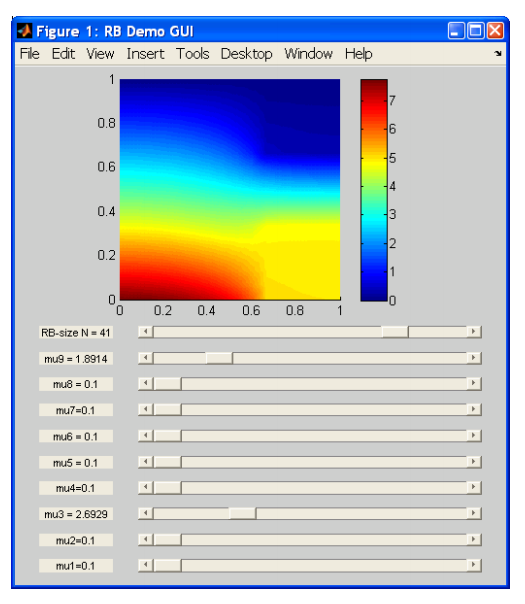
\includegraphics[width = 0.7 \textwidth]{Bilder/ThermoBlock.png}
  \caption{Beispiel des Thermischen Blocks aus \textsf{demo\_thermalblock.m}}{(aus B. Haasdonk, Reduzierte-Basis-Methoden, Skript zur Vorlesung SS 2011, Universität Stuttgart, IANS-Report 4/11, 2011.)}
  \label{fig:ThermoBlock}
\end{figure}

\subsubsection*{Offline/Online Zerlegung}
\label{Offline/Online Zerlegung}

Typischerweise wird eine Verechnungsintensive Generierung des reduzierten Modells akzeptiert, sog. \emph{Offline-Phase}. Dies ermöglicht schnelle Anwendbarkeit des reduzierten Modells in der \emph{Online-Phase}. Offline-Kosten werden gerechtfertigt durch Amortisierung im multi-query-Kontext, d.\,h. Laufzeitgewinn bei genügend großer Anzahl an Online-Simulationen

\begin{figure}[H]
  \centering\small
    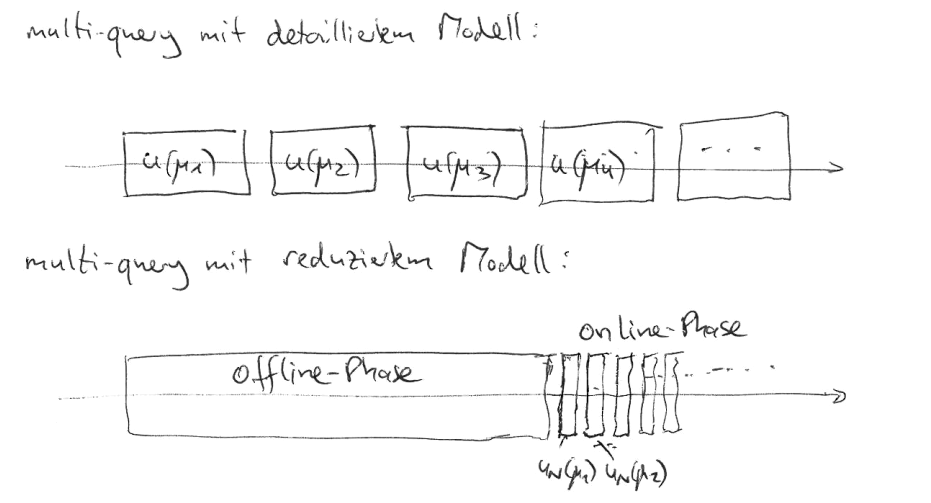
\includegraphics[width = 0.6 \textwidth]{Bilder/OfflineOnline.png}
  \caption{Laufzeitvergleich eines detaillierten mit einem reduzierten Modell}{(aus dem Online-Skript von Prof. Dr. Haasdonk zu Reduzierte Basen 2015)}
  \label{fig:OfflineOnline}
\end{figure}

\subsubsection*{Zentrale Fragen}
\label{Zentrale Fragen}

\begin{itemize}
	\item Reduzierte Basis: Wie kann ein möglichst kompakter Teilraum konstruiert werden? Können solche Verfahren \emph{beweisbar} gut sein?
	\item Reduziertes Modell: Wie kann eine Lösung $u_N(\mu) \in X_N$ bestimmt werden
	\item Berechnungs-Effizienz: Wie kann $u_N(\mu)$ \emph{schnell} berechnet wreden?
	\item Stabilität: Wie kann Stabilität des reduzierten Modells garantiert werden bei wachsendem $N := \text{dim } X_N$?
	\item Fehlerschätzer: Kann der Fehler des reduzierten zum detaillierten oder analytischen modells beschränkt werden? Sind die Fehlerschätzer schnell berechenbar?
	\item Effektivität der Fehlerschätzer: Kann garantiert werden, dass der Schätzer den Fehler nicht zu pessimistisch überschätzt?
	\item Für welche Problemklassen kann ein RB-Ansatz funktionieren, für welche nicht?
\end{itemize}

\subsubsection*{Vorläufige Gliederung}
\label{Vorläufige Gliederung}

\begin{enumerate}[1]
	\item Einleitung
	\item Grundlagen
	\item RB Verfahren für lineare koerzive Probleme
	\item Allgemeinere lineare Probleme
	\item Nichtlineare Probleme
	\item Instationäre Probleme
	\item Weiterführende Aspekte
\end{enumerate}